\documentclass{deltares_memo}
\usepackage{CJKutf8}
\newcommand{\menuarrow}{$\rightarrow$}
\newcommand{\plotcfts}{PlotCFTS\xspace}
\newcommand{\dflowfm}{D-Flow FM\xspace}
\newcommand{\qumesh}{QGIS\_UMESH\xspace}
\newcommand{\qgis}{QGIS\xspace}
\newcommand{\netcdf}{netCDF\xspace}
\newcommand{\cfstandard}{Climate and Forecast 1.7 standard\xspace}

\begin{document}
\memoTo{To whom it may concern}
\memoConfidentialUntil{}
\memoDate{\today}
\memoVersion{001}
\memoFrom{Jan Mooiman}
\memoTelephone{---}
\memoEmail{jan.mooiman@deltares nl}
\memoSubject{Manual to plot result files of \dflowfm in QGIS 3.14 (map- and history-files)}
\memoCopy{}

\deltarestitle

\tableofcontents

%--------------------------------------------------------------------------------
\section{Release Notes}
\phantom{m}\vspace{-\baselineskip}
%
%--- begin light blue table ---
\begin{longtable}{p{16mm-12pt}|p{\textwidth-16mm-12pt}} 
%\caption{Light blue theme of table} \\% 
\rowcolor{dblue1} 
\textbf{Release} 
& \textbf{Description} 
\\ 
\topline 
\endfirsthead 
\endhead 
\endfoot 
\bottomline 
\endlastfoot 
0.11.00  &  - Reading \file{$\ast$\_net.nc} file repaired.  \\
0.10.00  &  - Export to QGIS layer enabled for scalar quantities.  \\
0.00.00  &  - No information available.  \\
\end{longtable} 
%--- end light blue table ---
%
%--------------------------------------------------------------------------------
\section{Menu bar}
\phantom{m}\vspace{-\baselineskip}
\begin{figure}[H]
    \centering    
    \includegraphics[width=0.40\textwidth]{pictures/menu_bar.png}
    \caption{The menu bar of the \qumesh plugin}
\end{figure}

%------------------------------------------------------------------------------
\subsection{File}
\phantom{m}\vspace{-\baselineskip}
\begin{figure}[H]
    \centering    
    \includegraphics[width=0.40\textwidth]{pictures/menu_file.png}
    \caption{Menu \menuarrow File}
\end{figure}

%--------------------------------------------------------------------------------
\subsubsection{Open UGRID}
When selecting this option you are able to select \netcdf files which are meet the UGRID standard. 
Example files are the mesh- and map-file of the \dflowfm program (\file{$\ast$\_net.nc}, \file{$\ast$\_map.nc}).
Only the map-file could contain time series.
%--------------------------------------------------------------------------------
\subsubsection{Open HisCF}
When selecting this option you are able to select \netcdf files which are meet the climate and forecast history file standard.
Example files are the history output files of the program \dflowfm (\file{$\ast$\_his.nc}).
%--------------------------------------------------------------------------------
\subsection{Output}
\phantom{m}\vspace{-\baselineskip}
\begin{figure}[H]
    \centering    
    \includegraphics[width=0.40\textwidth]{pictures/menu_output.png}
    \caption{Menu \menuarrow Output}
\end{figure}

%------------------------------------------------------------------------------
\subsubsection{Show map output}
After selecting \menu{Output\menuarrow Show map output} the window \window{Map Output Animation} will open, see as example \autoref{fig:map_output_a}.
\begin{figure}[H]
\begin{subfigure}[b]{0.48\textwidth}
	\centering    
	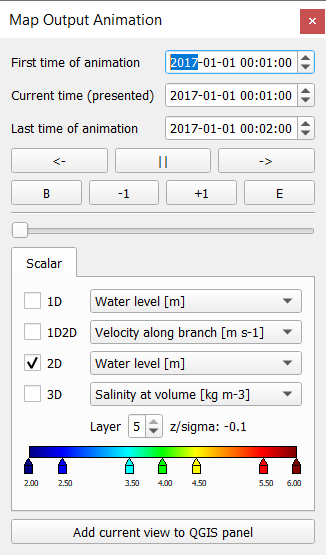
\includegraphics[width=\textwidth]{pictures/map_output_animation_window_scalar.png}
	\caption{Layout scalar quantities; sigma layer at $\sigma = -0.1$ (near the surface)\label{fig:map_output_a}}
	% file used for this picture: ugrid_1d2d3d_map.nc
\end{subfigure}
\hfill
\begin{subfigure}[b]{0.48\textwidth}
	\centering    
	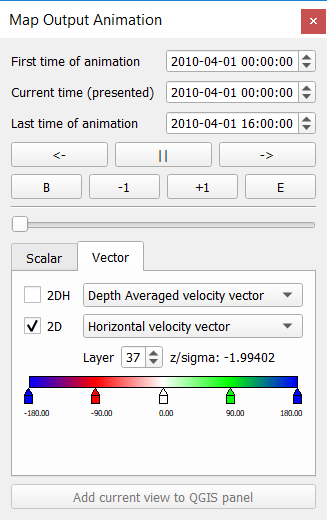
\includegraphics[width=\textwidth]{pictures/map_output_animation_window_vector.png}
	\caption{Layout vector quantities; fixed layer at $z = -1.99402$ (near the surface).}
\end{subfigure}    
    \caption{\window{Map Output Animation} window for scalars and vector.}
	% file used for this picture: agulhas_map.nc
\end{figure}
%------------------------------------------------------------------------------
\subparagraph*{Add current view to QGIS layer panel}
\Note This button is only enabled for scalar quantities.

After pressing the button \button{Add current view to QGIS panel} a window \window{Add current view to QGIS layer panel} will appear.
In this window you can specify the layer name which will be presented in the QGIS layer panel, see \autoref{fig:currentviewlayerpanel}
\begin{figure}[H]
	\centering    
	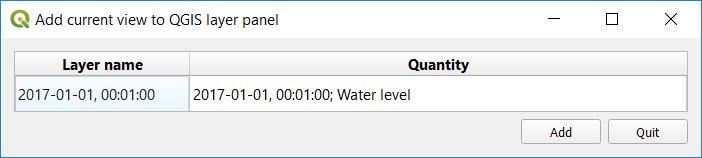
\includegraphics[width=0.90\textwidth]{pictures/current_view_add.png}
	\caption{Window \window{Add current view to QGIS layer panel}\label{fig:currentviewlayerpanel}}
\end{figure}
After pressing the button \button{Add} the layer will be added to the layer panel.
Pressing the \button{Quit} button will close the window.
%------------------------------------------------------------------------------
\subsubsection{PlotCFTS}
After selecting \menu{Output\menuarrow \plotcfts} the program \plotcfts will start, see as example \autoref{fig:plotcfts_main}.
Select from the menubar of the \plotcfts program menu option \menu{Help \menuarrow User Manual} to open the user manual for the program \plotcfts. 

\begin{figure}[H]
    \centering    
    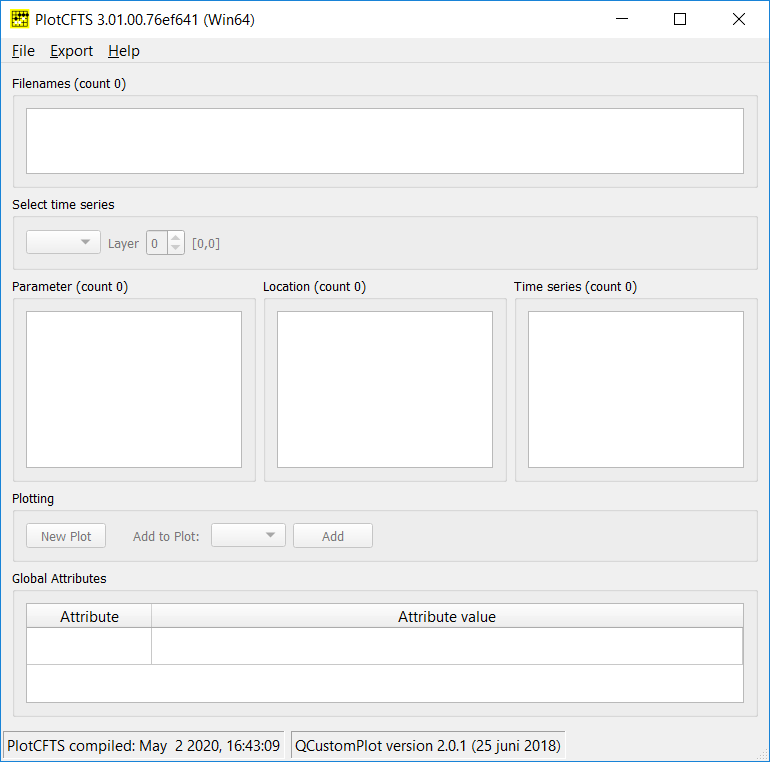
\includegraphics[width=0.9\textwidth]{pictures/main_plotcfts.png}
    \caption{Main window of the \plotcfts program.\label{fig:plotcfts_main}}
\end{figure}
%--------------------------------------------------------------------------------
\subsection{Settings}
Settings for the presentation of scalars and vectors.
\begin{figure}[H]
    \centering    
    \includegraphics[width=0.40\textwidth]{pictures/menu_settings.png}
    \caption{Menu \menuarrow Settings}
\end{figure}
When selecting this option some settings for the presentation of the variables via the window \window{Map Output Animation} can be set. 
This window will also pop up when using the right mouse button within the window \window{Map Output Animation}.
\begin{figure}[H]
	\centering    
	\includegraphics[width=0.50\textwidth]{pictures/map_properties.png}
	\caption{Window \window{Map Output Settings}\label{fig:map_output_settings}}
\end{figure}
The following quantities can be specified in the window presented by \autoref{fig:map_output_settings}:
\begin{longtable}{p{35mm-12pt} p{\textwidth-35mm-12pt}} 
	Transparency & Specify the transparency of the iso patches for the scalars. \\
	Refresh rate & Specify the refresh rate, in seconds, of the images during animation. \\	
	\textbf{Colorramp limits} & \\
	\textsl{Dynamic colorramp} & \\
	\underline{checked} & Colorramp limits are determined by the minimum and maximum value of the scalar. 
	These values reach their extreme values after all timestep are visualised.\\
	\underline{unchecked} & 
	Minimum value: \quad specify the minimum value for the scalar.\newline
	Maximum value: \quad specify the maximum value for the scalar.\\
	\textbf{Vector scaling} & \\
	Vector scaling & The vector of length 1 (ex.\ \SI{1}{\metre\per\second}) is scaled with this factor. The drawing length is based on the averaged cell size.
\end{longtable}
%--------------------------------------------------------------------------------
\subsection{Help}
\phantom{m}\vspace{-\baselineskip}
\begin{figure}[H]
    \centering    
    \includegraphics[width=0.4\textwidth]{pictures/menu_help.png}
    \caption{Menu \menuarrow Help}
\end{figure}

%--------------------------------------------------------------------------------
\subsubsection{User Manual}
Shows the user manual
\begin{figure}[H]
	\centering    
	\includegraphics[width=0.9\textwidth]{pictures/menu_help_user_manual.png}
	\caption{\qumesh user manual}
\end{figure}

%--------------------------------------------------------------------------------
\subsubsection{About}
Shows the about box.
\begin{figure}[H]
    \centering    
    \includegraphics[width=0.4\textwidth]{pictures/menu_help_about.png}
    \caption{About box}
\end{figure}
%--------------------------------------------------------------------------------
%\subsection{Trials}
%\phantom{m}\vspace{-\baselineskip}
%\begin{figure}[H]
%    \centering    
%    \includegraphics[width=0.40\textwidth]{pictures/menu_trials.png}
%    \caption{Menu \menuarrow Trials}
%\end{figure}
%------------------------------------------------------------------------------
\section{QGIS panels}
Some \qgis panels are shown after reading a \netcdf map-file.
%------------------------------------------------------------------------------
\subsection{Layer panel}
\begin{figure}[H]
	\centering    
	\includegraphics[width=0.4\textwidth]{pictures/panel_layers.png}
	\caption{The \qgis layer panel after reading a \netcdf map-file.\label{fig:panel_layer}}
\end{figure}
%------------------------------------------------------------------------------
\subsection{Log messages panel}
\begin{figure}[H]
	\centering    
	\includegraphics[width=0.95\textwidth]{pictures/panel_log_message.png}
	\caption{The \qgis layer panel after reading a \netcdf map-file.\label{fig:panel_layer}}
\end{figure}
%------------------------------------------------------------------------------
\section{Examples figures}
Examples are given for a scalar field (Depth averaged velocity magnitude) and the corresponding vector field (arrow and direction).
%------------------------------------------------------------------------------
\subsection{Example scalar field}
These fields are given on the output files of \dflowfm.
\begin{figure}[H]
	\centering    
	\includegraphics[width=0.95\textwidth]{pictures/oosterschelde_velocity_magnitude.png}
	\caption{Depth averaged velocity, magnitude.\label{fig:velocity_magnitude}}
\end{figure}
%------------------------------------------------------------------------------
\subsection{Example vector field}
These fields are not given on the output files of \dflowfm.
So the postprocessing program (\qumesh) need to compute the quantities of the vector field, like vector arrows and vector direction. 

\Note the "velocity magnitude" is given on the output file of \dflowfm and thus computed by \dflowfm.
The quantity "velocity magnitude" is therefor available in the tab \menu{Scalar}
\begin{figure}[H]
	\centering    
	\includegraphics[width=0.95\textwidth]{pictures/oosterschelde_velocity_arrow.png}
	\caption{Depth averaged velocity, vector.\label{fig:velocity_vector}}
\end{figure}

\begin{figure}[H]
	\centering    
	\includegraphics[width=0.95\textwidth]{pictures/oosterschelde_velocity_direction.png}
	\caption{Depth averaged velocity, direction.\label{fig:velocity_vector_direction}}
\end{figure}
%------------------------------------------------------------------------------
\section{Source}
The source code is available on GitHUB:

\url{https://github.com/Deltares/qgis_umesh}
%------------------------------------------------------------------------------

\end{document}
